\subsection{Motivation}
\begin{frame}{Research objectives}

\begin{block}{Aim}
    To identify the effect of differences in group com-position on learning effectiveness in two dimensions-i.e.  interaction between group  members  and  group  achievement-based  on  measurements  proposed by some previous studies.
\end{block}

\begin{alertblock}{Sub-research questions}
    \begin{enumerate}
    \item What are the overall patterns of knowledge transfer from individual-to-group representation?
    \item Does similarity of knowledge affect students' learning
    effectiveness in the two dimensions (i.e. interaction of individual 
    members and group level), and, if so, to what extent?
    \item Does similarity of knowledge affect the experiences of
    participants in the study, and, if so, to what extent?
\end{enumerate}
\end{alertblock}

%% The study focuses on identifying the effectiveness from the end-products 
%% (collaborative maps), the patterns of map changes from individuals to groups, 
%% and the perceptions of the students while following the learning activities. 
\end{frame}

\subsection{Analysis methods}
\begin{frame}{Variables involved in this study}
    \begin{figure}[tb]
     \begin{center}
      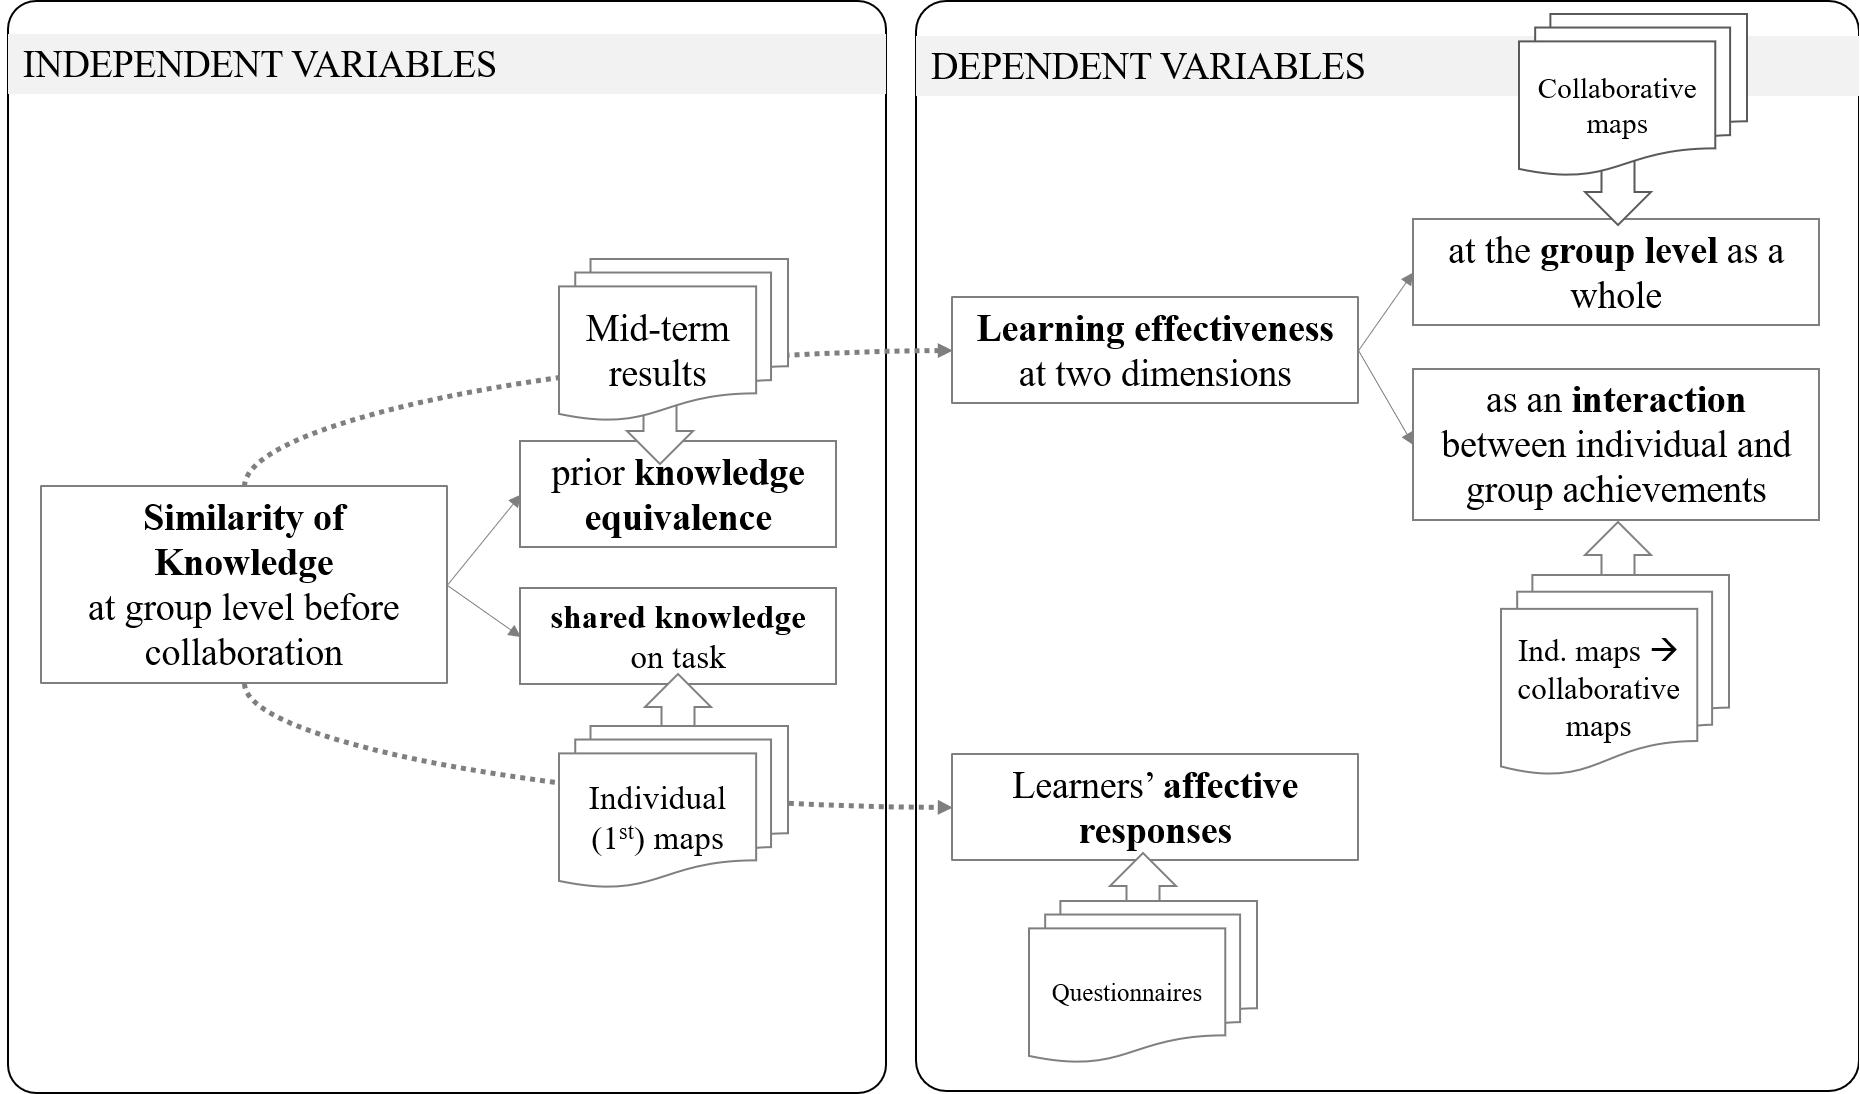
\includegraphics[width=120mm]{images/rqb_variables.pdf}
      \end{center}
      \caption{Variables involved in this study}
      \label{variables}  
\end{figure}
\end{frame}

\begin{frame}
    \begin{figure}[tb]
     \begin{center}
      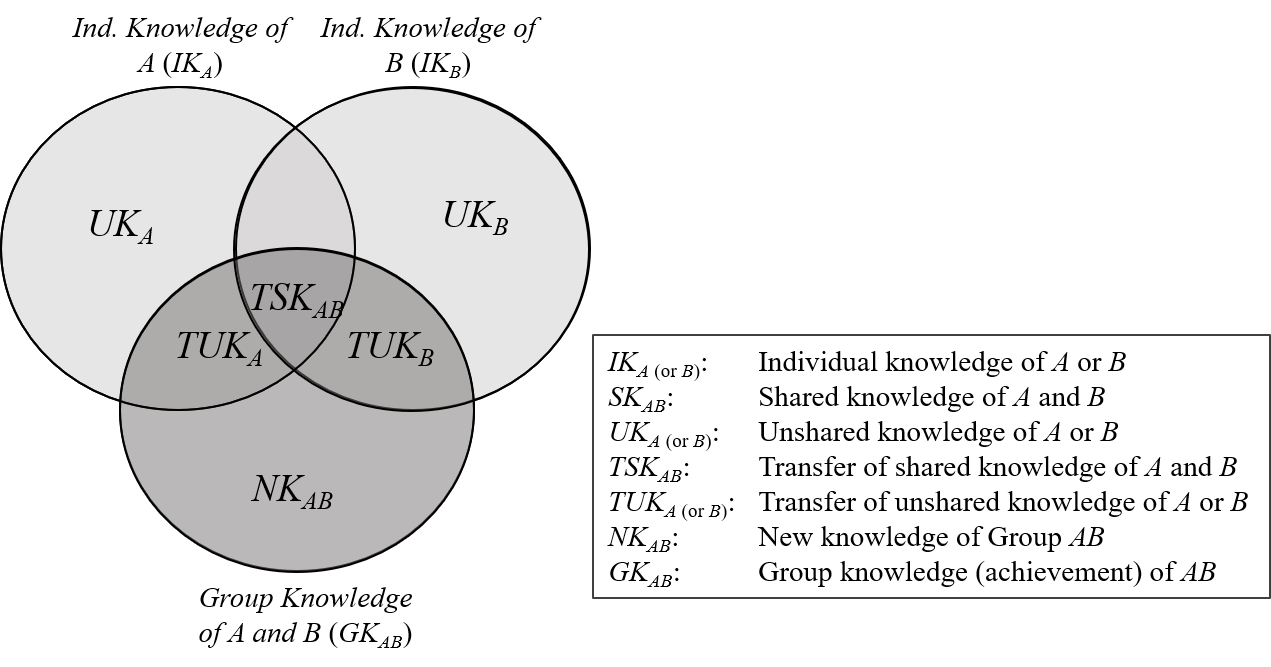
\includegraphics[width=120mm]{images/rqb_learn-effective.pdf}
      \end{center}
      \caption{Illustration of learning effectiveness analysis}
      \label{learn-effective}  
    \end{figure}
\end{frame}

\subsection{Results \& discussions}
\begin{frame}[allowframebreaks]{Results}
    \begin{figure}[tb]
     \begin{center}
      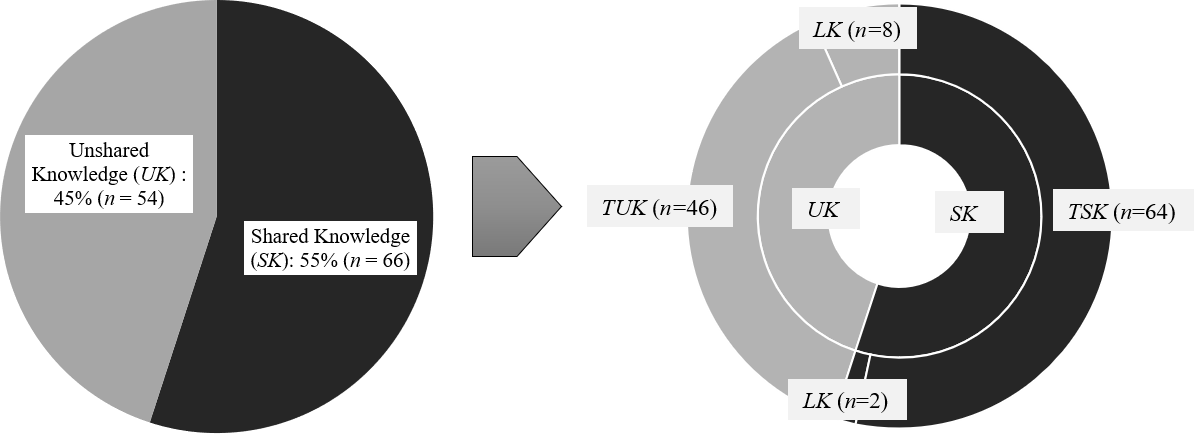
\includegraphics[width=120mm]{images/rqb_dist-knowledge.pdf}
      \end{center}
      \caption{Distribution  of  shared  and  unshared  knowledge  in  individual maps prior to collaboration (left) and distribution of individual knowledge transferred to collaborative maps in all groups (right)}
      \label{learn-effective}  
    \end{figure}
    
    \begin{figure}[tb]
     \begin{center}
      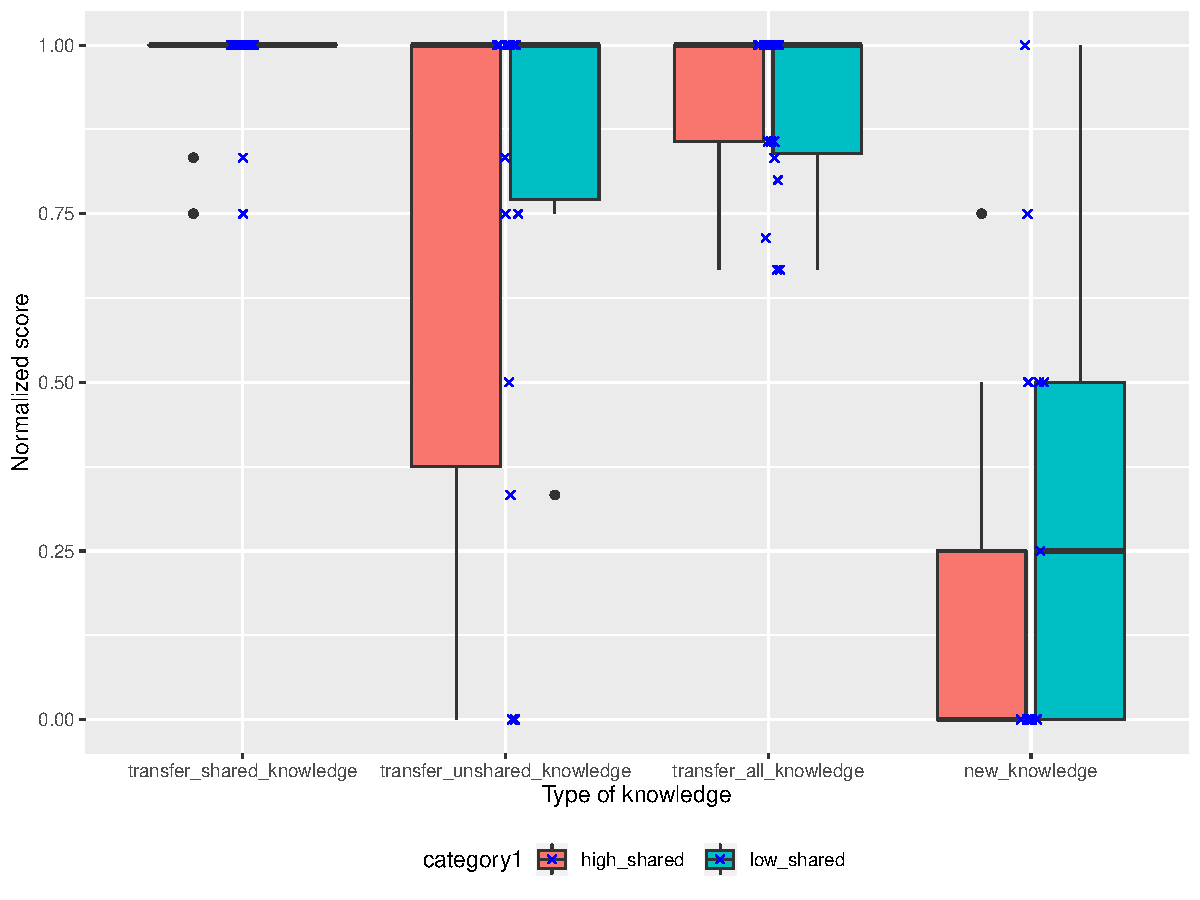
\includegraphics[width=120mm]{images/rqb_dist-shared-all-redraw.pdf}
      \end{center}
      \caption{Distribution of knowledge transfer and new knowledge in high-and  low-prior-knowledge-equivalence  groups}
      \label{learn-effective}  
    \end{figure}

\end{frame}
    
\begin{frame}[allowframebreaks]{Results 2}
    \begin{figure}[tb]
     \begin{center}
      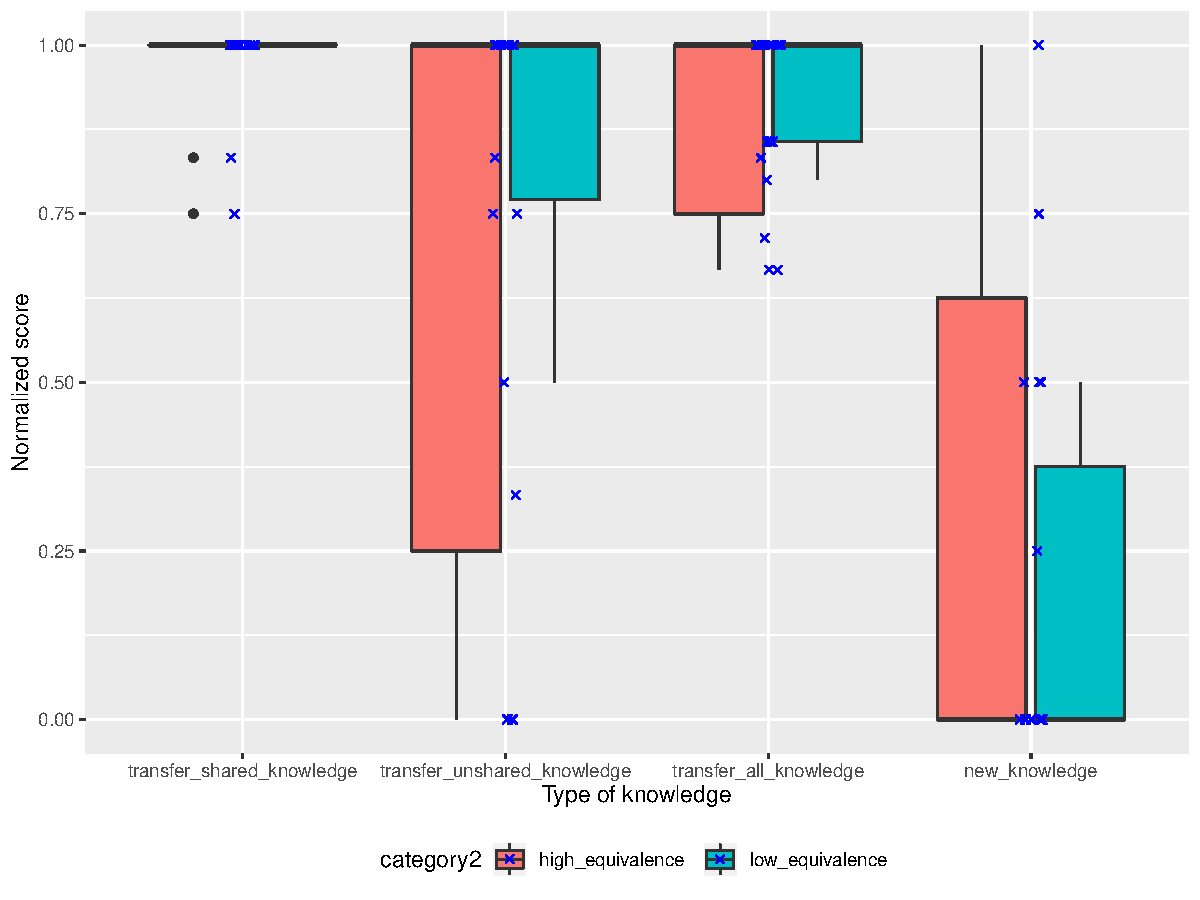
\includegraphics[width=120mm]{images/rqb_dist-equivalence-all-redraw.pdf}
      \end{center}
      \caption{Distribution of knowledge transfer and new knowledge in high-and low-shared-knowledge groups}
      \label{learn-effective}  
    \end{figure}
    
    \begin{figure}[tb]
     \begin{center}
      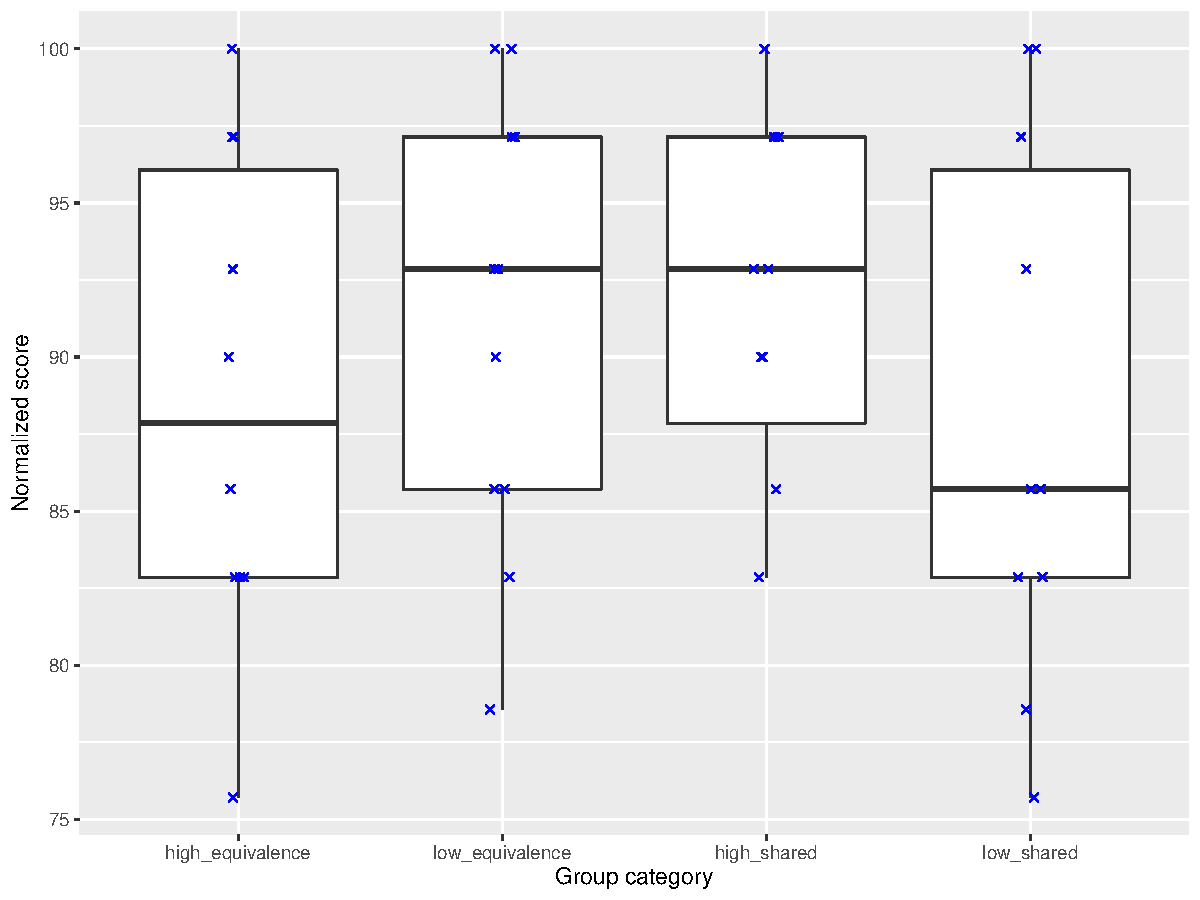
\includegraphics[width=120mm]{images/rqb_group-map-redraw.pdf}
      \end{center}
      \caption{Collaborative map scores differentiated by prior-knowledge 
      equivalence and shared knowledge about the task}
      \label{group-map}  
    \end{figure}
\end{frame}

\begin{frame}[allowframebreaks]{Results 3}
    \begin{figure}[tb]
     \begin{center}
      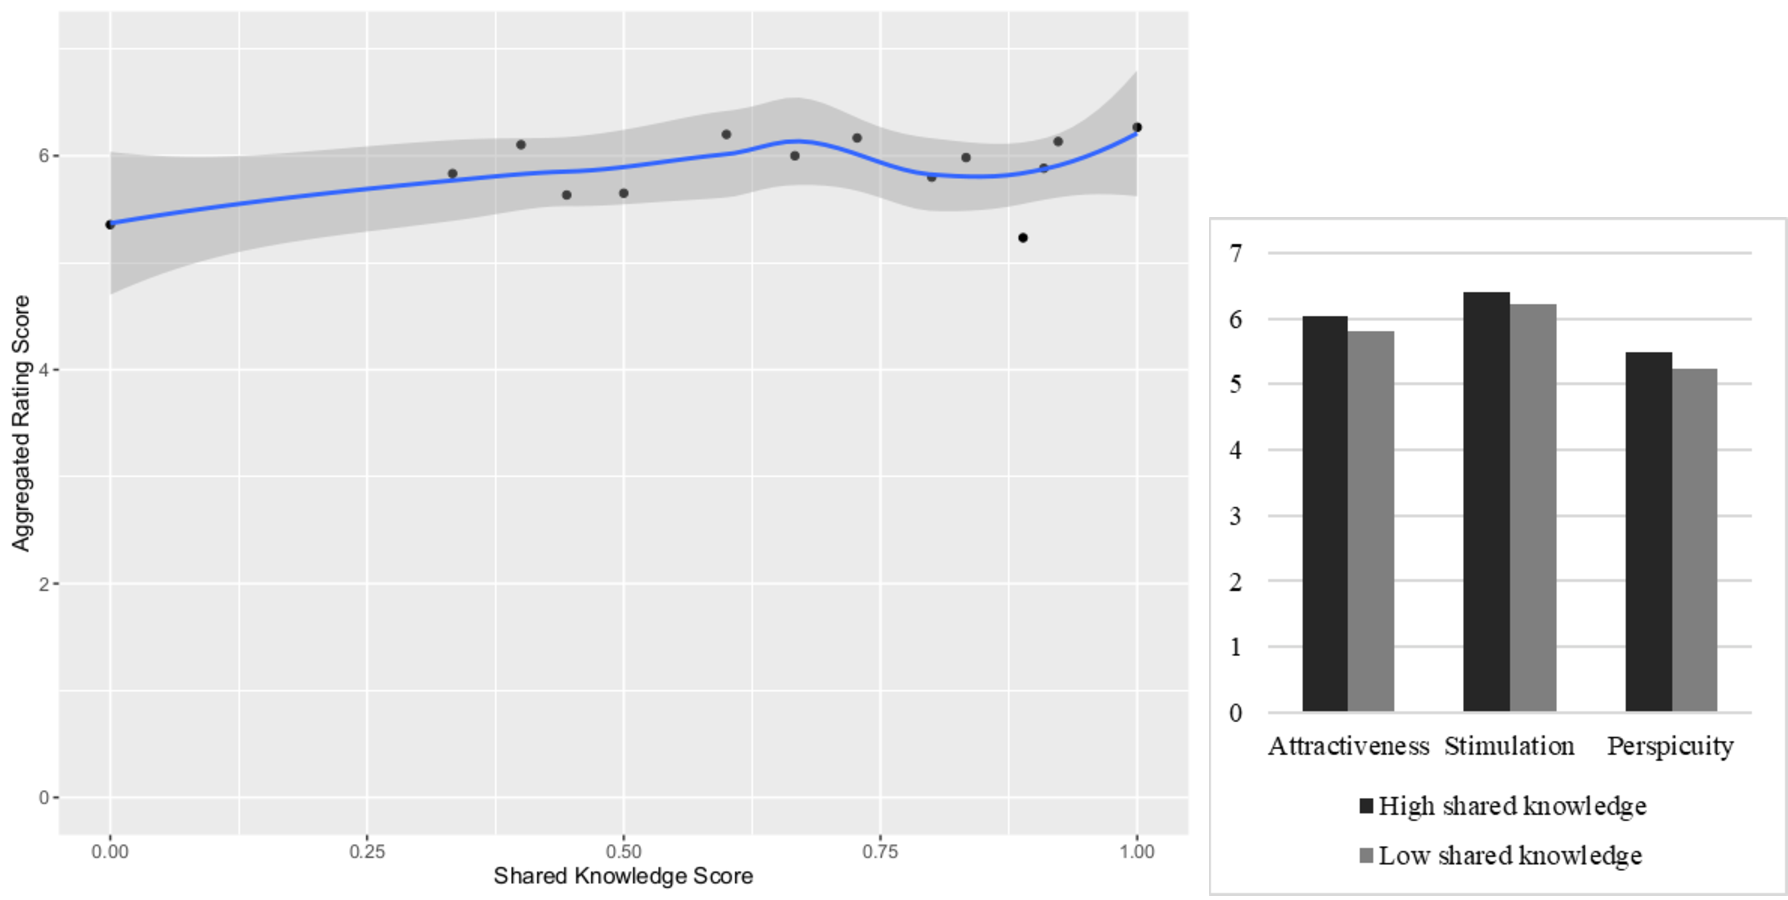
\includegraphics[width=120mm]{images/rqb_affective-response-redraw.pdf}
      \end{center}
      \caption{Distribution  of  affective  responses  across  different  shared-knowledge scores}
      \label{learn-effective}  
    \end{figure}
\end{frame}
